\section{Organisation des transactions}

This chapter opens the «~micro~» half of the course. It starts with the questions
economics is asked today and with a first picture of how an economy is organised:
the circuit économique, which links the ménages and the entreprises through two
kinds of market; the frontière des possibilités de production, which bounds what an
economy can produce; and three complexités that make the economy hard to
understand. One example, the price of a coffee in a station or an airport, then
shows economic reasoning at work, and its answer is not the obvious one.\\

The second part asks how transactions are organised. Prices have to be set, and
there are two approaches: a decentralised one, by négociations bilatérales or
multilatérales or by an automated mechanism, and a centralised one, under which the course files
both Marx and the market. What
négociations bilatérales cost, and the debate between Marx and Hayek, close the
chapter.

\subsection{Les grandes questions d'aujourd'hui}

Three great questions of today, each with the themes it raises (IA stands for
intelligence artificielle).

\begin{itemize}
  \item \textbf{IA, emploi et transition numérique} --- thèmes~: croissance et
    innovation, économie du travail, compétences, inégalités, protection de la vie
    privée~;
  \item \textbf{Changement climatique et transition écologique} --- thèmes~:
    pollution = externalité négative, coordination internationale~;
  \item \textbf{Inflation, dette et risques financiers} --- pouvoir de marché et
    concurrence, bulles financières, pouvoir d'achat, impôts, politiques
    monétaires.
\end{itemize}

\subsection{Comprendre l'économie}

Three diagrams first picture the economy as a whole --- the circuit économique,
then the frontière des possibilités de production before and after a shift; three
complexités then say why it is hard to understand.\\

The \textbf{circuit économique} (\textit{circular flow}) strips the economy down to
two kinds of agent and two kinds of market. Only the ménages and the entreprises
take decisions in it. On the \textbf{marchés des biens et services}
(\textit{markets for goods and services}) the entreprises are the sellers and the
ménages the buyers; on the \textbf{marchés des facteurs de production}
(\textit{markets for the factors of production}) the roles are reversed, with the
ménages selling and the entreprises buying. The \textbf{facteurs de production}
(\textit{factors of production}) --- le travail, la terre et le capital --- belong
to the ménages; the entreprises hire them and use them to produce the biens et
services they sell, which the ménages buy and consume.\\

Against every flow of biens et services or of facteurs de production runs a flow of
money in the opposite direction. What the ménages spend on the marchés des biens et
services, their dépenses, reaches the entreprises as recettes; what the entreprises
pay on the marchés des facteurs de production, as salaires, loyers et profits,
reaches the ménages as revenus.\\

\begin{figure}[h!]
  \centering
  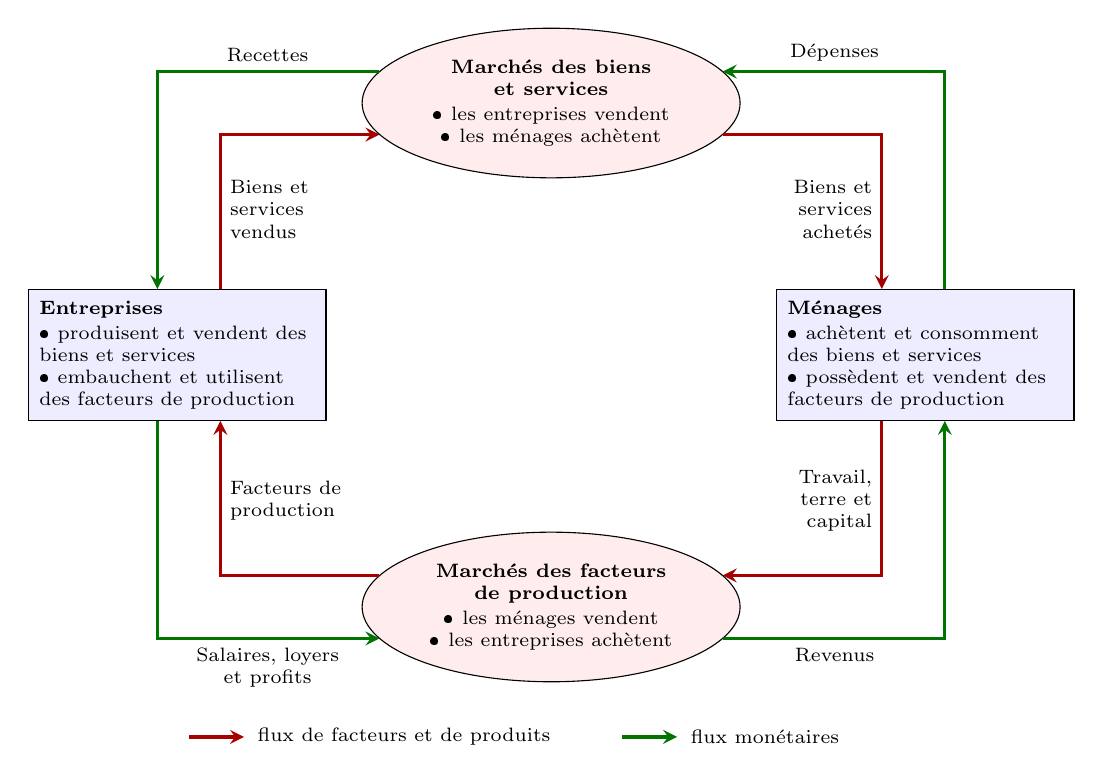
\begin{tikzpicture}[font=\scriptsize, >=stealth,
      real/.style={->, very thick, red!65!black},
      money/.style={->, very thick, green!45!black}]
    % the two markets
    \draw[fill=red!7] (0,3.2) ellipse (2.4 and 0.95);
    \node[align=center] at (0,3.2) {\textbf{Marchés des biens}\\\textbf{et services}\\[1pt]
      \textbullet{} les entreprises vendent\\\textbullet{} les ménages achètent};
    \draw[fill=red!7] (0,-3.2) ellipse (2.4 and 0.95);
    \node[align=center] at (0,-3.2) {\textbf{Marchés des facteurs}\\\textbf{de production}\\[1pt]
      \textbullet{} les ménages vendent\\\textbullet{} les entreprises achètent};
    % the two agents
    \node[draw, fill=blue!7, text width=3.5cm, align=left, inner sep=4pt] (E) at (-4.75,0)
      {\textbf{Entreprises}\\[1pt]
       \textbullet{} produisent et vendent des biens et services\\
       \textbullet{} embauchent et utilisent des facteurs de production};
    \node[draw, fill=blue!7, text width=3.5cm, align=left, inner sep=4pt] (M) at (4.75,0)
      {\textbf{Ménages}\\[1pt]
       \textbullet{} achètent et consomment des biens et services\\
       \textbullet{} possèdent et vendent des facteurs de production};
    \coordinate (li) at (-4.2,0); \coordinate (lo) at (-5.0,0);
    \coordinate (ri) at (4.2,0);  \coordinate (ro) at (5.0,0);
    % inner loop: goods and factors
    \draw[real] (li |- E.north) |- (-2.18,2.8);
    \draw[real] (2.18,2.8) -| (ri |- M.north);
    \draw[real] (ri |- M.south) |- (2.18,-2.8);
    \draw[real] (-2.18,-2.8) -| (li |- E.south);
    % outer loop: money
    \draw[money] (-2.18,3.6) -| (lo |- E.north);
    \draw[money] (ro |- M.north) |- (2.18,3.6);
    \draw[money] (2.18,-3.6) -| (ro |- M.south);
    \draw[money] (lo |- E.south) |- (-2.18,-3.6);
    % labels of the flows
    \node[above] at (-3.6,3.6) {Recettes};
    \node[above] at (3.6,3.6) {Dépenses};
    \node[right, align=left] at (-4.2,1.85) {Biens et\\services\\vendus};
    \node[left, align=right] at (4.2,1.85) {Biens et\\services\\achetés};
    \node[right, align=left] at (-4.2,-1.85) {Facteurs de\\production};
    \node[left, align=right] at (4.2,-1.85) {Travail,\\terre et\\capital};
    \node[below, align=center] at (-3.6,-3.6) {Salaires, loyers\\et profits};
    \node[below] at (3.6,-3.6) {Revenus};
    % legend
    \draw[real] (-4.6,-4.85) -- (-3.9,-4.85);
    \node[right] at (-3.85,-4.85) {flux de facteurs et de produits};
    \draw[money] (0.9,-4.85) -- (1.6,-4.85);
    \node[right] at (1.65,-4.85) {flux monétaires};
  \end{tikzpicture}
  \caption*{\small Le circuit économique. The ménages and the entreprises take the
  decisions and meet on the two kinds of market. The inner arrows are the flows of
  facteurs de production and of biens et services; the outer arrows are the
  corresponding flows of money, running the other way round.}
\end{figure}

The \textbf{frontière des possibilités de production} (\textit{production
possibilities frontier}) is drawn here for voitures and ordinateurs, and it
separates what the economy can produce of the two goods from what it cannot. The
attainable combinations are those on the frontière itself, such as $A$, $B$, $E$
and $F$, and those inside it, such as $D$. A point beyond it, such as $C$, asks for
more than the economy's resources can deliver.\\

Suppose now that the technology for making ordinateurs improves. Whatever number of
voitures the economy turns out, it can now make more ordinateurs than before, and
the whole frontière moves outward: on the ordinateurs axis it now starts at
$4\,000$ instead of $3\,000$, while on the voitures axis it still ends at $1\,000$.
From $A$ ($600$ voitures, $2\,200$ ordinateurs) the economy can then move to $G$
($650$ voitures, $2\,300$ ordinateurs), with more of both goods.\\

\begin{figure}[h!]
  \centering
  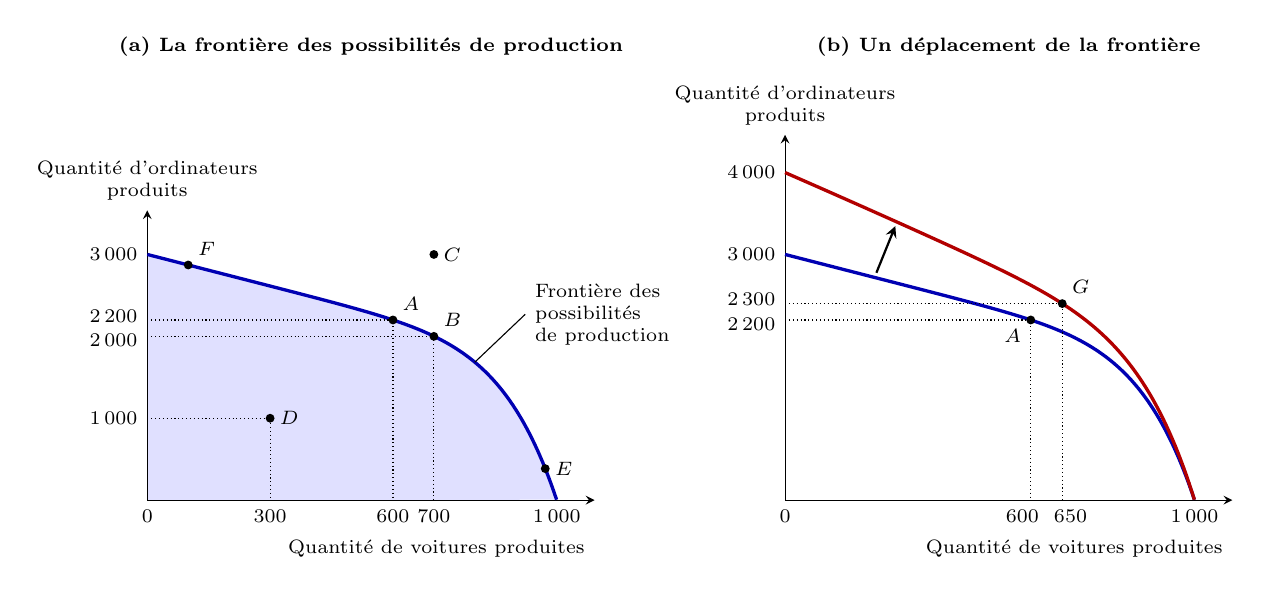
\begin{tikzpicture}[x=0.8cm, y=0.8cm, font=\scriptsize, >=stealth,
      ttl/.style={align=center, font=\scriptsize\bfseries},
      xlab/.style={anchor=north east, yshift=-11pt},
      declare function={ppf(\x) = 3.9*(1 - 0.42845*\x/6.5 - 0.57155*(\x/6.5)^8);}]
    % (a) the frontier
    \begin{scope}
      \node[ttl] at (3.55,7.2) {(a) La frontière des possibilités de production};
      \fill[blue!12] (0,0) -- plot[domain=0:6.5, samples=150] (\x, {ppf(\x)}) -- cycle;
      \draw[->] (0,0) -- (7.1,0);
      \draw[->] (0,0) -- (0,4.6);
      \node[xlab] at (7.1,0) {Quantité de voitures produites};
      \node[above, align=center] at (0,4.6) {Quantité d'ordinateurs\\produits};
      \draw[very thick, blue!70!black]
        plot[domain=0:6.5, samples=150] (\x, {ppf(\x)});
      % guides and ticks
      \draw[densely dotted] (0,2.86) -| (3.9,0);
      \draw[densely dotted] (0,2.6) -| (4.55,0);
      \draw[densely dotted] (0,1.3) -| (1.95,0);
      \node[below] at (0,0) {$0$};
      \node[below] at (1.95,0) {$300$};
      \node[below] at (3.9,0) {$600$};
      \node[below] at (4.55,0) {$700$};
      \node[below] at (6.5,0) {$1\,000$};
      \node[left] at (0,1.3) {$1\,000$};
      \node[left, yshift=-1.5pt] at (0,2.6) {$2\,000$};
      \node[left, yshift=1.5pt] at (0,2.86) {$2\,200$};
      \node[left] at (0,3.9) {$3\,000$};
      % points
      \fill (0.65,3.733) circle (1.6pt) node[above right] {$F$};
      \fill (3.9,2.86) circle (1.6pt) node[above right] {$A$};
      \fill (4.55,2.6) circle (1.6pt) node[above right] {$B$};
      \fill (6.318,0.5) circle (1.6pt) node[right] {$E$};
      \fill (1.95,1.3) circle (1.6pt) node[right] {$D$};
      \fill (4.55,3.9) circle (1.6pt) node[right] {$C$};
      % name of the curve
      \draw (5.2,2.19) -- (6.0,2.95);
      \node[right, align=left] at (6.0,2.95) {Frontière des\\possibilités\\de production};
    \end{scope}
    % (b) its shift
    \begin{scope}[xshift=8.1cm]
      \node[ttl] at (3.55,7.2) {(b) Un déplacement de la frontière};
      \draw[->] (0,0) -- (7.1,0);
      \draw[->] (0,0) -- (0,5.8);
      \node[xlab] at (7.1,0) {Quantité de voitures produites};
      \node[above, align=center] at (0,5.8) {Quantité d'ordinateurs\\produits};
      % initial frontier (blue) and new frontier (red)
      \draw[very thick, blue!70!black]
        plot[domain=0:6.5, samples=150] (\x, {ppf(\x)});
      \draw[very thick, red!70!black]
        plot[domain=0:6.5, samples=150]
          (\x, {ppf(\x) + 1.3*(1 - \x/6.5)*(1 + 0.1034*\x/6.5)});
      \draw[->, thick] (1.45,3.61) -- (1.75,4.35);
      % guides and ticks
      \draw[densely dotted] (0,2.86) -| (3.9,0);
      \draw[densely dotted] (0,3.12) -| (4.4,0);
      \node[below] at (0,0) {$0$};
      \node[below, xshift=-3pt] at (3.9,0) {$600$};
      \node[below, xshift=3pt] at (4.4,0) {$650$};
      \node[below] at (6.5,0) {$1\,000$};
      \node[left, yshift=-1.5pt] at (0,2.86) {$2\,200$};
      \node[left, yshift=1.5pt] at (0,3.12) {$2\,300$};
      \node[left] at (0,3.9) {$3\,000$};
      \node[left] at (0,5.2) {$4\,000$};
      % points
      \fill (3.9,2.86) circle (1.6pt) node[below left] {$A$};
      \fill (4.4,3.12) circle (1.6pt) node[above right] {$G$};
    \end{scope}
  \end{tikzpicture}
  \caption*{\small La frontière des possibilités de production entre voitures et
  ordinateurs (a) et son déplacement (b). In (a) the shaded set is what the economy
  can produce; $C$, outside it, is not attainable with the economy's resources. In
  (b) a technological advance in the production of ordinateurs shifts the frontière
  outward, from the blue curve to the red one; the voitures intercept does not move.
  From $A$ to $G$ the economy produces more voitures and more ordinateurs. The ticks
  near $A$ and $G$ are spread for legibility, not drawn to scale.}
\end{figure}

Three complexités make the economy hard to understand.

\begin{itemize}
  \item \textbf{Première complexité~: tout est interconnecté.} The notion it calls
    for is the \textbf{équilibre général} (\textit{general equilibrium}), and the example
    given is the crise de 2008.
  \item \textbf{Deuxième complexité~: le futur détermine le présent.} It has two
    sides. First, the rôle des \textbf{anticipations} (\textit{expectations}):
    \textbf{prophéties auto-réalisatrices} (\textit{self-fulfilling prophecies})
    and \textbf{anticipations rationnelles} (\textit{rational expectations}).
    Second, the \textbf{arbitrage intertemporel} (\textit{intertemporal
    trade-off}): investissement / production, épargne / consommation,
    innovations.
  \item \textbf{Troisième complexité~: les agents économiques ont des informations
    différentes.} These are the \textbf{asymétries d'information}
    (\textit{information asymmetries}). The question «~Pourquoi faire une
    transaction financière~?~» is raised with them and left open.
\end{itemize}

\subsection{Comprendre les enjeux économiques à travers un exemple}

One example shows how an economist reads a price: why does a coffee cost so much
in a station or an airport? The two obvious answers, une demande forte or une
demande captive, turn out to be the wrong ones. The argument rests on one quantity.

\begin{definition}[Marge (\textit{markup})]
  La \textbf{marge}~: markup = prix – coût marginal.
\end{definition}

\begin{example}[Le prix d'un café dans une gare]
  «~Pourquoi le prix d'un café est si cher dans une gare ou dans un aéroport~?~»
  --- «~Une demande forte~? Une demande captive~?~» The argument answers by a chain
  of questions.
  \begin{enumerate}
    \item \emph{D'où vient la marge~?} For a coffee it is «~environ 150 cents~».
      It comes from two sources, and each is a \textbf{choix stratégique}
      (\textit{strategic choice}). The first is where the kiosk stands,
      «~position du kiosque à café à l'intersection de différents couloirs ou seul
      à la fin d'une allée (terminal aéroport)~», and «~la position n'est pas
      aléatoire (exogène), c'est un choix stratégique (endogène)~». The second is
      «~l'absence de concurrents~: choix stratégique (endogène)~».
    \item \emph{Pourquoi est-ce qu'il n'y a pas de concurrents~?} The kiosk is a
      \textbf{monopole local} (\textit{local monopoly}). The cost of
      entry does not explain it, since the \textbf{coûts fixes d'entrée}
      (\textit{fixed costs of entry}) are low: «~ce n'est pas très coûteux de
      monter un kiosque à café (le marché est contestable, avec des coûts fixes
      d'entrée faibles)~».
    \item \emph{Réponse avec une autre question~: qui gagne de l'argent~?}
      «~L'employé~? La chaîne qui possède le kiosque~?~» --- «~Aucun des deux~»~:
      «~le propriétaire qui loue les locaux commerciaux~».
    \item \emph{Le choix stratégique du propriétaire d'espaces dans la gare ou
      l'aéroport.} The owner can «~louer des emplacements commerciaux à beaucoup de
      kiosques qui se font concurrence~», or offer a single kiosk a
      \textbf{contrat d'exclusivité} (\textit{exclusive contract}). The answer is
      in the question: the contrat d'exclusivité lets the owner of the space take the surplus of the
      kiosk's owner, an \textbf{extraction du surplus} (\textit{surplus extraction}) ---
      «~extraction du surplus du propriétaire du kiosque~; exemple~: enchère au
      second prix~».
    \item \emph{Conclusion~: pourquoi un prix du café élevé~?} The price carries a
      \textbf{double marge de monopole} (\textit{double marginalisation}). La
      double marge de monopole provient de la rareté des espaces commerciaux~:
      «~C'est ce qui cause le prix élevé, pas la demande.~»
  \end{enumerate}
\end{example}

Two owners appear in the argument and must be kept apart: the owner of the
commercial space, who rents it out and earns the money, and the owner of the
kiosk, whose surplus the first extracts through the contrat d'exclusivité. The position
of the kiosk and the absence of competitors are both endogène, the outcome of
choices; the high price follows from the rareté des espaces commerciaux, not from
the demand of the travellers.

\subsection{Comment organiser les transactions ?}

«~Il faut déterminer des prix~»; there are two approaches.

\begin{itemize}
  \item \emph{Décentralisée.}
    \begin{itemize}
      \item \textbf{Négociations bilatérales} (\textit{bilateral negotiations})
        / multilatérales. Problème~: facturation à la tête du client ---
        \textbf{discrimination par les prix} (\textit{price discrimination}) ---
        ou en fonction du \textbf{pouvoir de négociation} (\textit{bargaining
        power}).
      \item Automatisée~: exemple~: marché de l'énergie décentralisée, P2P
        lending.
    \end{itemize}
  \item \emph{Centralisée.}
    \begin{itemize}
      \item Marx.
      \item Le marché~: concurrence parfaite.
    \end{itemize}
\end{itemize}

As the classification stands, the market, in its concurrence parfaite form, falls
under the centralised approach, beside Marx. The two are set against each other in
Marx vs.\ Hayek below.

\subsubsection{Négociations bilatérales}

Organising exchange by négociations bilatérales runs into three problems.

\begin{itemize}
  \item Les \textbf{coûts de transaction} (\textit{transaction costs}), notion due à
    Ronald Coase~: ils expliquent la taille des entreprises.
  \item Les problèmes des \textbf{contrats incomplets} (\textit{incomplete
    contracts})~: des risques informationnels --- la sélection adverse et l'aléa
    moral.
  \item Les négociations bilatérales n'exploitent pas les économies d'échelle.
\end{itemize}

Sélection adverse and aléa moral are only named here, and the course does not
develop them; the asymétries d'information return with the défaillances de marché,
through Akerlof's lemons alone.

\subsection{Marx vs.\ Hayek}

The two centralised forms of the classification above face each other here: Marx
on one side, the market on the other. The case for the market is put, with
Hayek and l'école de Chicago, as «~le marché résout la complexité de la
centralisation et agrège l'information~». La notion de valeur et de prix is raised
alongside it.\\

The discussion then asks «~et avec l'IA~?~» --- in context, whether intelligence
artificielle could make centralisation work. The answer is «~sans doute non~», and
two points come with it:

\begin{itemize}
  \item «~critères de redistribution~?~», a question left open;
  \item les informations privées des agents économiques.
\end{itemize}
